% Options for packages loaded elsewhere
\PassOptionsToPackage{unicode}{hyperref}
\PassOptionsToPackage{hyphens}{url}
%
\documentclass[10pt,a4paper]{article}
\usepackage[left=25mm,right=25mm]{geometry}
\usepackage{amsmath}
\usepackage{amsfonts}
\usepackage{amssymb}

\author{}
\date{}



\usepackage{listings}
\usepackage{color}

\definecolor{dkgreen}{rgb}{0,0.6,0}
\definecolor{gray}{rgb}{0.5,0.5,0.5}
\definecolor{mauve}{rgb}{0.58,0,0.82}

\lstset{frame=tb,
  language=C,
  aboveskip=3mm,
  belowskip=3mm,
  showstringspaces=false,
  columns=flexible,
  basicstyle={\small\ttfamily},
  numbers=none,
  numberstyle=\tiny\color{gray},
  keywordstyle=\color{blue},
  commentstyle=\color{dkgreen},
  stringstyle=\color{mauve},
  breaklines=true,
  breakatwhitespace=true,
  tabsize=3
}

\usepackage{multicol}
\usepackage{graphicx}
\usepackage{epstopdf}

\epstopdfDeclareGraphicsRule{.gif}{png}{.png}{convert gif:#1 png:\OutputFile}
\AppendGraphicsExtensions{.gif}
\usepackage{chngcntr}
\counterwithin*{equation}{section}
\counterwithin*{equation}{subsection}
\usepackage{amsmath}

\usepackage{float} 
\usepackage{hyperref}
\usepackage{amsmath}
\let\oldsubsection\subsection
\renewcommand{\subsection}{%
    \setcounter{equation}{0}%
    \oldsubsection%
}
\begin{document}


\begin{flushleft}
\begin{LARGE}EE 435 Homework 2 Spring 2024
\end{LARGE}
\\Jonathan Hess
\\\href{https://github.com/Jetsama/EE435/tree/main/HW2}{GitHub Page}
\end{flushleft}


\subsection*{Problem 1 and 2}
Consider the following operational amplifier. The goal is to obtain an
expression for the small-signal output voltage in terms of the input variables INV+ and INV-.\\
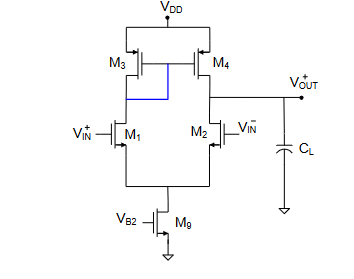
\includegraphics[width=3in]{images/Problem1.png} \\


\subsubsection*{a)}
Write a complete set of small-signal equations that can be solved to obtain
\(V_{OUT}\). Assume the small-signal parameter \(g_o\) is present in all MOS devices.\\


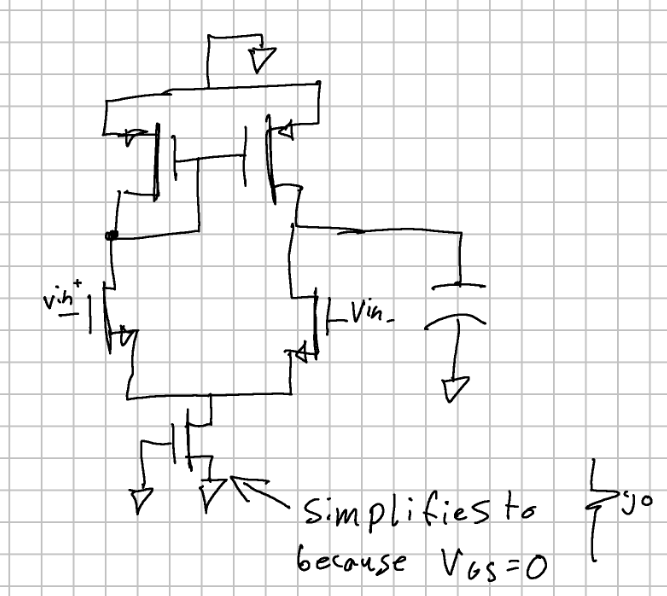
\includegraphics[width=3in]{images/p1p1.png} \\
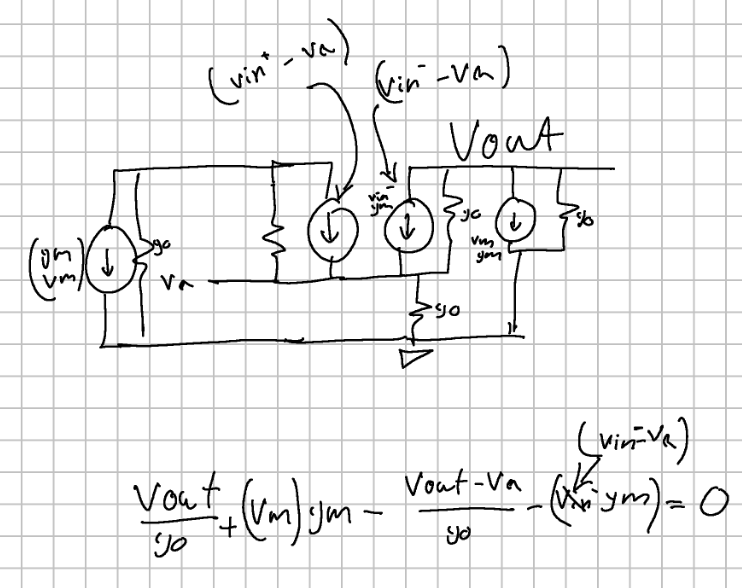
\includegraphics[width=3in]{images/p1p2.png} \\

Three equations are created via KCL analysis of the small signal model. They are as follows:\\

\[(V_{\text{out}} - V_{a}) \cdot g_0 + V_{\text{out}} \cdot g_0 + (V_{\text{inN}} - V_{a}) \cdot g_m + V_m \cdot g_m = 0\]

\[(V_m - V_{a}) \cdot g_0 + V_m \cdot g_0 + (V_{\text{inP}} - V_{a}) \cdot g_m + V_m \cdot g_m = 0\]

\[V_a \cdot g_0 + (V_a - V_m) \cdot g_0 + (V_a - V_{\text{out}}) \cdot g_0 - (V_{\text{inP}} - V_{a}) \cdot g_m - (V_{\text{inN}} - V_{a}) \cdot g_m = 0\]

\subsubsection*{b)}
Solve these equations by hand for \(V_{OUT}\). If you do not have a solution at
the end of ½ hour, stop, and comment on your progress and the amount of
effort that you believe would be required to finish the solution.\\

\textbf{INCORRECT}\\
NOTE: this is attempt was incorrect because I used go as resistance rather than conductance

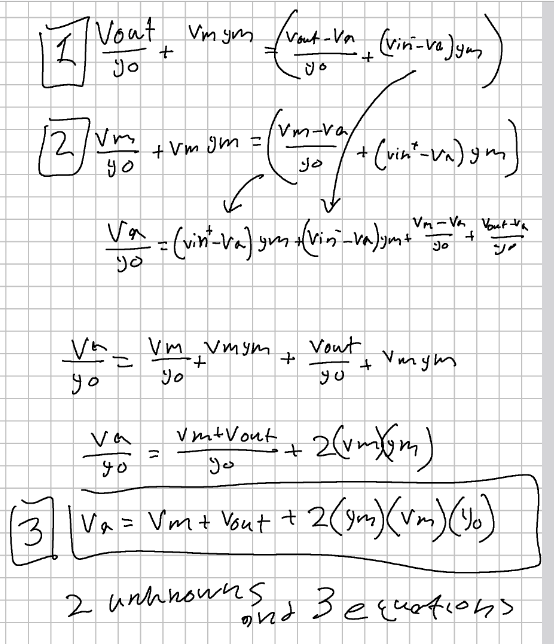
\includegraphics[width=3in]{images/p1p3.png} \\
\begin{equation}
\frac{V_{out}}{g_0} + (V_m) gm = \frac{V_{out} - V_a }{g_0} + V_{in-}g_m 
\end{equation}

\begin{equation}
\frac{V_{out}}{g_0} \frac{V_{out} - V_a }{g_0} = (V_m) gm + V_{in-}g_m 
\end{equation}
\begin{equation}
V_{out} * \frac{2}{g_0} = (V_{in-} + V_m - V_a)g_m +  \frac{V_{a}}{g_0}
\end{equation}

\begin{equation}
V_{out} = \frac{(V_{in-} + V_m - V_a)g_m}{2} +  \frac{V_{a}}{2}
\end{equation}



\begin{equation}
V_{m} = (\frac{-V_{out}}{g_0} + V_{in-}g_m) * \frac{1}{\frac{1}{g_0} - g_m + 2g_m^2g_0}
\end{equation}

\begin{equation}
V_{a} = V_m + V_{out} + 2(g_m)(V_m)(g_0)
\end{equation}

\begin{equation}
V_{a} = V_{out} + V_m( 1+ 2(g_m)(g_0))
\end{equation}


Now replace all $V_a$ in the VOUT equation.

\begin{equation}
V_{out} = \frac{(V_{in-} + V_{out} - 2(g_m)(V_m)(g_0))g_m}{2} +  \frac{V_m + V_{out} + 2(g_m)(V_m)(g_0)}{2}
\end{equation}
Now replace all $V_m$ in the  equation.
\begin{multline}
V_{out} = \frac{(V_{in-} + V_{out} - 2(g_m)((\frac{-V_{out}}{g_0} + V_{in-}g_m) * \frac{1}{\frac{1}{g_0} - g_m + 2g_m^2g_0})(g_0))g_m}{2}\\ +  \frac{(\frac{-V_{out}}{g_0} + V_{in-}g_m) * \frac{1}{\frac{1}{g_0} - g_m + 2g_m^2g_0} + V_{out} + 2(g_m)((\frac{-V_{out}}{g_0} + V_{in-}g_m) * \frac{1}{\frac{1}{g_0} - g_m + 2g_m^2g_0})(g_0)}{2}
\end{multline}
At this point I spent way to much time on this problem. So I moved onto part c. I then realized that I was using g0 as a resistance rather than conductance.\\
\textbf{CORRECTED}\\



\subsubsection*{c)}
Obtain a parametric (symbolic) solution for the transfer function \(V_{OUT}/V_{IN}\)
from this set of equations with MATLAB. How many total product terms appear in this
solution? In this part, \(V_{IN} = V_{IN+} - V_{IN-}\).\\

\begin{lstlisting}
syms Vm Va Vout go gm Vin VinN VinP

eq1 = (Vout-Va)*go + Vout*go + (VinN-Va)*gm +Vm*gm  == 0;
eq2 = (Vm-Va)*go + Vm*go + (VinP-Va)*gm +Vm*gm  == 0;
eq3 = Va*go + (Va-Vm)*go +(Va-Vout)*go - (VinP-Va)*gm - (VinN-Va)*gm == 0;
eq4 = Vin == VinP-VinN;

out = solve([eq1,eq2,eq3,eq4], [Vout,Vm,VinP,VinN,Va])
out.Vout

\end{lstlisting}
\begin{lstlisting}

ans =
 
(2*Vin*gm^2 + Vin*go*gm)/(4*go*(gm + go))\end{lstlisting}


\begin{equation}
\frac{V_{out}}{V_{in}} = \frac{(2 * g_m^2) + (g_m g_0) }{4 g_0 (g_m + g_0)}
\end{equation}

\subsubsection*{d)}
Simplify the solution obtained with MATLAB under the assumption that all \(g_o\) terms are small compared to \(g_m\) terms.\\

\begin{equation}
\frac{V_{out}}{V_{in}} =\frac{g_m}{2 g_0}
\end{equation}











\subsection*{Problem 3}
A transresistance amplifier with a gain \(R_T\) is shown. Derive an expression
for the voltage gain of the amplifier as a function of the transresistance gain \(R_T\) and determine what that reduces to if \(R_T\) is very large.\\
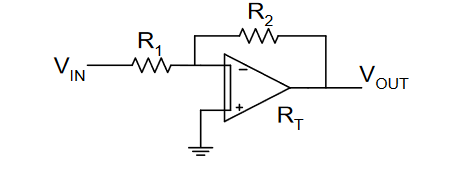
\includegraphics[width=6in]{images/Problem3.png} \\


In this circuit we are using a transresistance amplifier which has a gain of $V_{out} = R_f * i_{in}$. The $i_{in}$ for this circuit is $\frac{V_{in}}{R_1}$ because $V_{neg}$ is a virtual ground. We can then do a KVL. 
\begin{equation}
\frac{V_{in}}{R_1} + \frac{V_{out}}{R_2} - i_{in}= 0
\end{equation}

\begin{equation}
\frac{V_{in}}{R_1} + \frac{V_{out}}{R_2} - \frac{V_{out}}(R_f)= 0
\end{equation}

\begin{equation}
\frac{V_{in}}{R_1} =  V_{out}  * \frac{R_2 -R_f}{R_2*R_f}
\end{equation}

\begin{equation}
\frac{V_{out}}{V_{in}} =  \frac{R_2*R_f}{R_1(R_2 -R_f)}
\end{equation}



\begin{equation}
lim_{R_f \to \infty} \frac{R_2*R_f}{R_1(R_2 -R_f)} = \frac{R_2}{R_1}
\end{equation}
	
	
	
	
	
	
	
	
	

\subsection*{Problem 4}
Assume the amplifier shown below is designed in a 0.18$\mu$ CMOS process.
Assume also that \(V_{DD} = 1V\), \(V_{SS} = -1V\), and \(I_{DQ} = 4mA\).\\
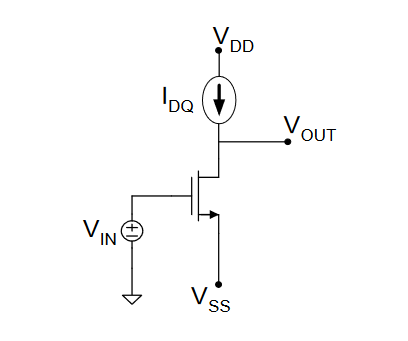
\includegraphics[width=3in]{images/Problem4.png} \\

\subsubsection*{a)}
Analytically determine the \(W\) and \(L\) needed to establish a quiescent output
voltage of 0.5V when \(V_{INQ} = 0.5V\).\\

Since we are using a mosfet in linear (non saturation region), we can use the following equations:

\begin{equation}
i_{d} = K * (2(V_{GS} - V_{TN}) V_{DS} - V_{DS}^2)
\end{equation}
Where
\begin{equation}
K =\frac{1}{2}(\mu_n C_{ox})\frac{W}{L}
\end{equation}


\begin{equation}
V_{out} = V_{DS} + V_{SS}  = 0.5 V
\end{equation}

\begin{equation}
V_{DS} = 1.5 V
\end{equation}

\begin{equation}
V_{in} = V_{GS} - V_{SS} = 0.5 V
\end{equation}
\begin{equation}
V_{GS} = 1.5 V
\end{equation}

To get the W/L we can use the current:

\begin{equation}
i_{d} = K * (2(V_{GS} - V_{TN}) V_{DS} - V_{DS}^2)	
\end{equation}
To get the VTN, I used the reference sheet for the process. 
\begin{equation}
V_{TN} =  0.5V
\end{equation}


The output current of the amplifier is:
\begin{equation}
i_{d} = 4mA = K * (2(1.5 -0.5)(1.5V) - (1.5V)^2)
\end{equation}

\begin{equation}
i_{d} = 4mA = K * (2(1)(1.5V) - (1.5V)^2)
\end{equation}

\begin{equation}
4mA = K * (3 - 2.25)V
\end{equation}

\begin{equation}
4*10^{-3} A = K * 0.75V
\end{equation}

\begin{equation}
\frac{16}{3}*10^{-3} = K = \frac{1}{2}(\mu_n C_{ox})\frac{W}{L} = 171.8 \frac{uA}{V^2} \frac{W}{L}
\end{equation}

\begin{equation}
\frac{W}{L} = \frac{80000}{2577} \approx 31.04
\end{equation}



\subsubsection*{b)}
Verify the transfer characteristics by Spice simulation.

\subsubsection*{c)}
Analytically determine the dc voltage gain at the Q-point established in a).

\subsubsection*{d)}
Using SPICE, obtain a plot of the small signal voltage gain versus the
quiescent output voltage.

\subsection*{Problem 5 and 6}
Design a 5T op amp to have a dc gain of 50dB and a GB of 2MHz
in the ON 0.5$\mu$m CMOS process. Assume \(V_{DD} = 3.5V\) and \(C_L = 1pF\).
Assume also that the bias voltages \(V_{B1}\) and \(V_{B2}\) can be precisely set so that a CMFB circuit is not needed.
Verify the gain and the GB of your design with a SPICE simulation.\\
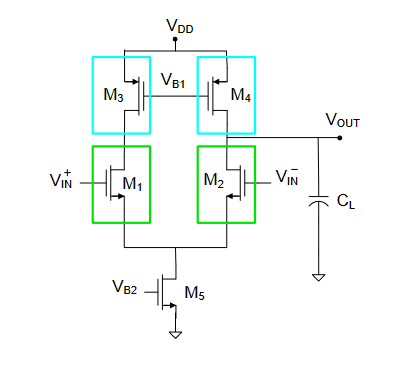
\includegraphics[width=4in]{images/Problem5.png} \\

We can use the equations given in the lecture slides.\\
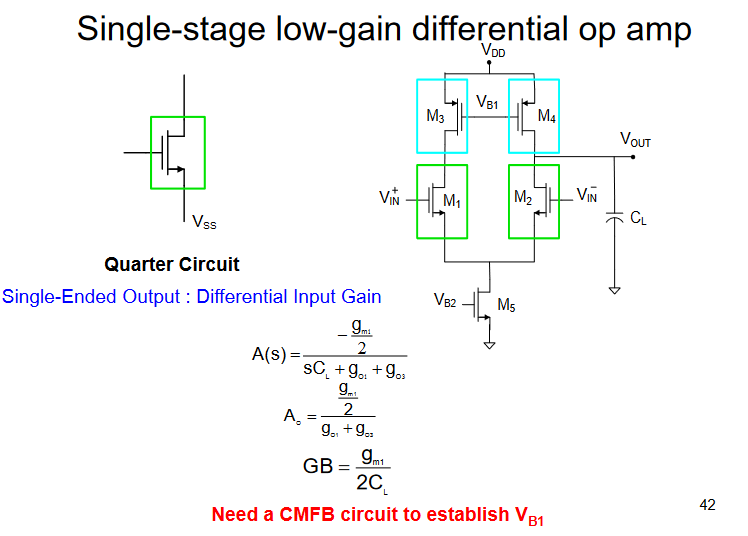
\includegraphics[width=4in]{images/5TOpamp.png} \\
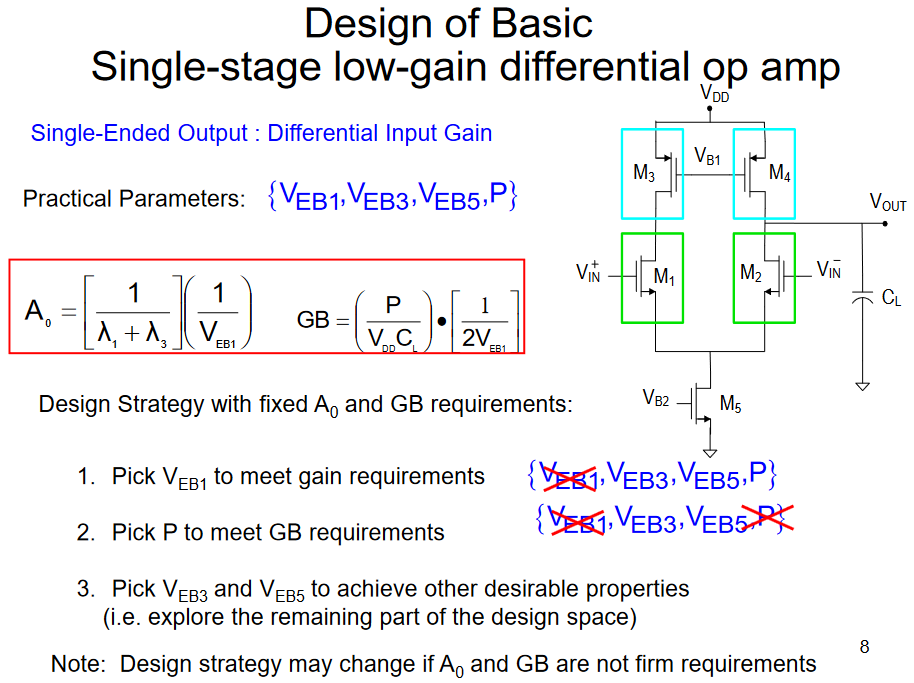
\includegraphics[width=4in]{images/5TOpampPractical.png} \\

First convert the $50dB = 10 log(\frac{V_{out}}{V_{in}})$. We then get that $A = 10^5$.


\begin{equation}
A = \frac{1}{\lambda_1 + \lambda_2} \frac{1}{V_{EB1}} = 10^5 =
\end{equation}


\begin{equation}
g_{mn} = (\mu_n C_{ox})\frac{W}{L} = 57.8*2 \frac{W}{L}
\end{equation}



\subsection*{Problem 7}
Determine the common-mode input range and the output signal swing of
the amplifier you designed in the previous problem.

\subsection*{Problem 8}
Assume that the op amp is a single-pole amplifier with gain given by the
expression \(A(s) = \frac{A_{0} \omega_A}{s + \omega_A} \approx \frac{GB}{s}\), where the gain-bandwidth product of the op amp is
\(GB = A_0\omega_A\). The right-most approximation to the gain is almost always justifiable whenused to characterize the operational amplifier since the gain of the op amp is so large at dc and since at frequencies even modestly above $/omega_A$, there is little difference between the middle term and the right term in this expression.\\

\subsubsection*{a)}
Assuming that the frequency-dependent gain of the op amp can be modeled as
\(A(s) \approx \frac{A_{GB}}{s}\), determine the transfer function
\(\frac{V_{OUT}}{V_{IN}}\) for the following two amplifiers.\\
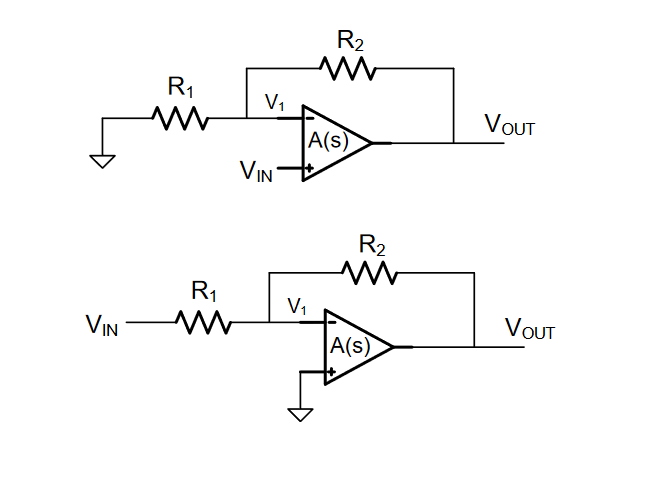
\includegraphics[width=6in]{images/Problem8.png} \\




\[
\frac{V_{OUT}}{V_{IN}} = \frac{A_{GB}}{s} \times \frac{1}{1 + \frac{1}{2}s}
\]



First for the first circuit we start with the following equations.
\begin{equation}
V_{out} = A(s)(V_{in} - V_N)
\end{equation}
\begin{equation}
V_N = \frac{V_{OUT}*R1}{R_1 + R_2}
\end{equation}
Then we can solve using the VN equation to replace VN in the original.
\begin{equation}
V_{out} = A(s)(V_{in} - \frac{V_{OUT}*R1}{R_1 + R_2})
\end{equation}
\begin{equation}
V_{out}(1 + \frac{R_1 * A(s)}{R_2 + R_1} = A(s)V_{in} 
\end{equation}

\begin{equation}
\frac{V_{out}}{V_{in}} = \frac{A(s)}{1+\frac{R_1 * A(s)}{R_2 + R_1}} 
\end{equation}
\begin{equation}
\frac{V_{out}}{V_{in}} = \frac{A(s)(R_1 + R_2)}{(R_1 + R_2) + R_1 * A(s)} 
\end{equation}
Now replace A(s)!
\begin{equation}
\frac{V_{out}}{V_{in}} = \frac{\frac{A_{GB}}{s}(R_1 + R_2)}{(R_1 + R_2) + R_1 * \frac{A_{GB}}{s}} 
\end{equation}

\begin{equation}
\frac{V_{out}}{V_{in}} = \frac{A_{GB}(R_1 + R_2)}{s(R_1 + R_2) + R_1 * A_{GB}} 
\end{equation}


Now for the second circuit we do a similar analysis.
\begin{equation}
V_{out} = A(s)(V_P - V_1)
\end{equation}
\begin{equation}
V_P = 0
\end{equation}
\begin{equation}
V_1 = Vout - \frac{(V_{out} - V_{in})R_2}{R_1+R_2}
\end{equation}

\begin{equation}
V_1 = Vin - \frac{(V_{in} - V_{out})R_1}{R_1+R_2}
\end{equation}

\begin{equation}
Vout - \frac{(V_{out} - V_{in})R_2}{R_1+R_2} = Vin - \frac{(V_{in} - V_{out})R_1}{R_1+R_2}
\end{equation}
The vout and VN



\subsubsection*{b)}
With the same op amp model used in part a), analytically determine the 3dB
bandwidth of the following two amplifiers.



\subsubsection*{c)}
Derive the gain of the inverting feedback amplifier in terms of \(A_{V}\) and \(\beta\) and
comment on why it does not look like the standard feedback equation.

\subsection*{Problem 9}
It was stated in class that all even-ordered distortion terms introduced by
the amplifier vanish in symmetric fully differential amplifiers. Prove this fact.

\subsection*{Problem 10 (Extra Credit)}
The “dead network” of a circuit is obtained by setting all small-signal inputs to 0. That is, by replacing all ac voltage sources with short circuits and all ac current sources with open circuits. The $\beta$ of a feedback amplifier is a characteristic of the “dead network”. Consider the basic inverting and noninverting feedback amplifiers shown below. These are widely used as small-signal voltage amplifiers.\\
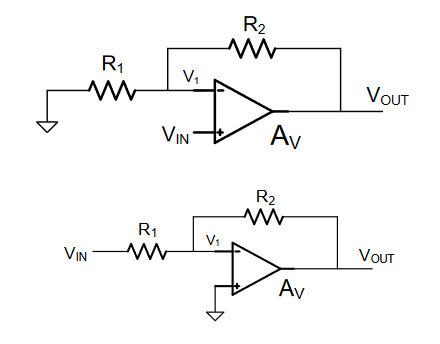
\includegraphics[width=6in]{images/Problem10.png} \\

\subsubsection*{a)}
Show that they both have the same “dead network”.

\subsubsection*{b)}
The \(\beta\) of the two amplifiers shown is \(\frac{1}{1 + \frac{R_1}{R_2}}\). Show that the gain of the
noninverting feedback amplifier can be expressed by the standard feedback
equation
\[
A = \frac{V_{OUT}}{V_{IN}} = \frac{1 + \frac{R_2}{R_1}}{\frac{R_2}{R_1}}
\]

\subsubsection*{c)}
Take the limit as \(A_V\) goes to $\infty$ for the gain derived in part b) and compare with
that derived in EE 230 for the gain of the noninverting feedback amplifier.

\subsubsection*{d)}
Derive the gain of the inverting feedback amplifier in terms of \(A_V\) and \(\beta\) and
comment on why it does not look like the standard feedback equation.




http://class.ece.iastate.edu/ee435/miscHandouts/TSMC%200.18%20T48K.pdf

http://class.ece.iastate.edu/ee330/lectures/EE%20330%20Lect%2025%20Fall%202023.pdf

\end{document}







